\documentclass[aspectratio=169, 14pt]{beamer}
\usepackage[utf8]{inputenc}
\usepackage[english]{babel}
\usepackage{tipa}
\usepackage{graphicx}
\usepackage{transparent}
\usepackage{multicol}
\usepackage[ruled, lined, linesnumbered, commentsnumbered]{algorithm2e}
\usepackage{pgfplots}
\newcommand\mycommfont[1]{\small\ttfamily\textcolor{blue}{#1}}
\SetCommentSty{mycommfont}
\renewcommand{\thealgocf}{}
\usepackage{setspace}
\usepackage{tikz}
\usetikzlibrary{matrix,backgrounds}
\usetikzlibrary{arrows}
\usetikzlibrary {arrows.meta}
\usetikzlibrary{calc,shadows.blur,fit,positioning}
\usetikzlibrary{shapes.multipart,chains}
\usepackage{minted}
\usepackage{fontawesome5}
\usepackage{booktabs}
\usepackage{caption}
\usepackage{bookmark}
\usepackage{hyperref}
\hypersetup{
    colorlinks=true,
    linkcolor=blue,
    filecolor=magenta,      
    urlcolor=cyan,
    }
\urlstyle{same}
\usetheme{metropolis}
\metroset{block=fill}
\usecolortheme{default}
\definecolor{darkmidnightblue}{rgb}{0.0, 0.2, 0.4}
\definecolor{LightGray}{gray}{0.9}


%------------------------------------------------------------
%This block of code defines the information to appear in the
%Title page
\title[Data Structures] %optional
{Data Structures}

\subtitle{Balanced Search Trees}

\author[CHEN Zhongpu] % (optional)
{CHEN Zhongpu}

\institute[] % (optional)
{
  School of Computing and Artificial Intelligence \\
  \href{mailto:zpchen@swufe.edu.cn}{zpchen@swufe.edu.cn}
}

\date[] % (optional)
{SWUFE, Fall 2022}

%End of title page configuration block
%------------------------------------------------------------


%------------------------------------------------------------
%The next block of commands puts the table of contents at the 
%beginning of each section and highlights the current section:

% \AtBeginSection[]
% {
%   \begin{frame}
%     \frametitle{Table of Contents}
%     \tableofcontents[currentsection]
%   \end{frame}
% }
%------------------------------------------------------------


\begin{document}

%The next statement creates the title page.
\frame{\titlepage}

%---------------------------------------------------------
%This block of code is for the table of contents after
%the title page
% \begin{frame}
% \frametitle{Table of Contents}
% \tableofcontents
% \end{frame}
%--------------------------------------------------------
\begin{frame}
    \frametitle{Small Quiz}
\begin{enumerate}
    \item Please draw the BST after inserting 4, 10, 8, 1, 2, and 7 sequentially.
    \item If we use an \emph{in-order} method to traverse it, what shall we see?
\end{enumerate}   

\end{frame}

\begin{frame}
    \frametitle{Small Quiz}

Please fill in the blank of the following algorithm.

    \scalebox{.8}{  
        \begin{algorithm}[H]
        \caption{get(key)}
        $x\gets root$ \\
    \While{x $\neq$ null and x.key $\neq$ key}{
        \If{\underline{\hspace{3cm}}}{
            $x\gets x.left$
        }\Else{
            $x\gets x.right$
        }
    }
    \Return{x}
    \end{algorithm}
    }
    

\end{frame}

{
    % \usebackgroundtemplate{\transparent{0.3}{\begin{picture}
    %     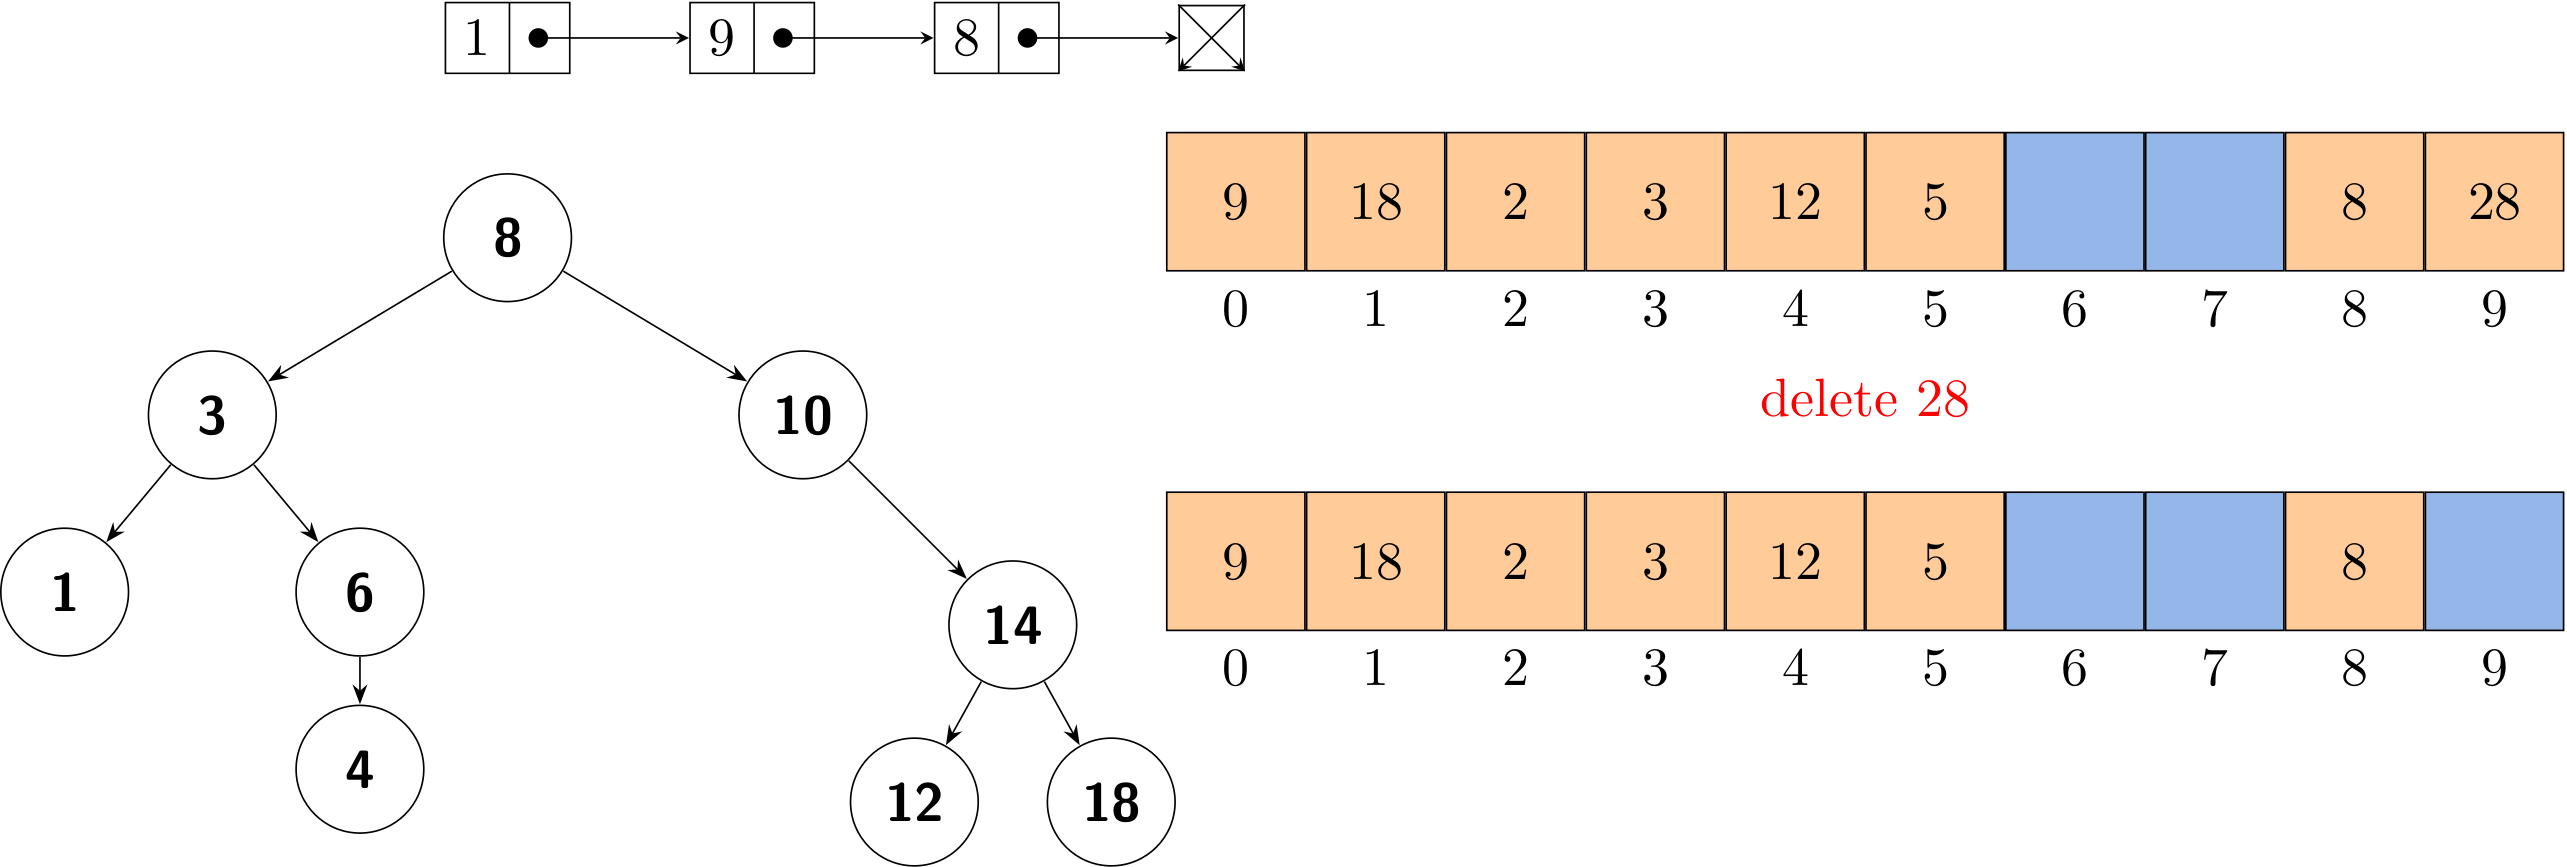
\includegraphics[height=0.7\paperheight]{cover}
    % \end{picture}    
    % }}
\usebackgroundtemplate{
  \tikz[overlay,remember picture] 
  \node[opacity=0.3, at=(current page.south east),anchor=south east, yshift=2cm,xshift=4cm] {
    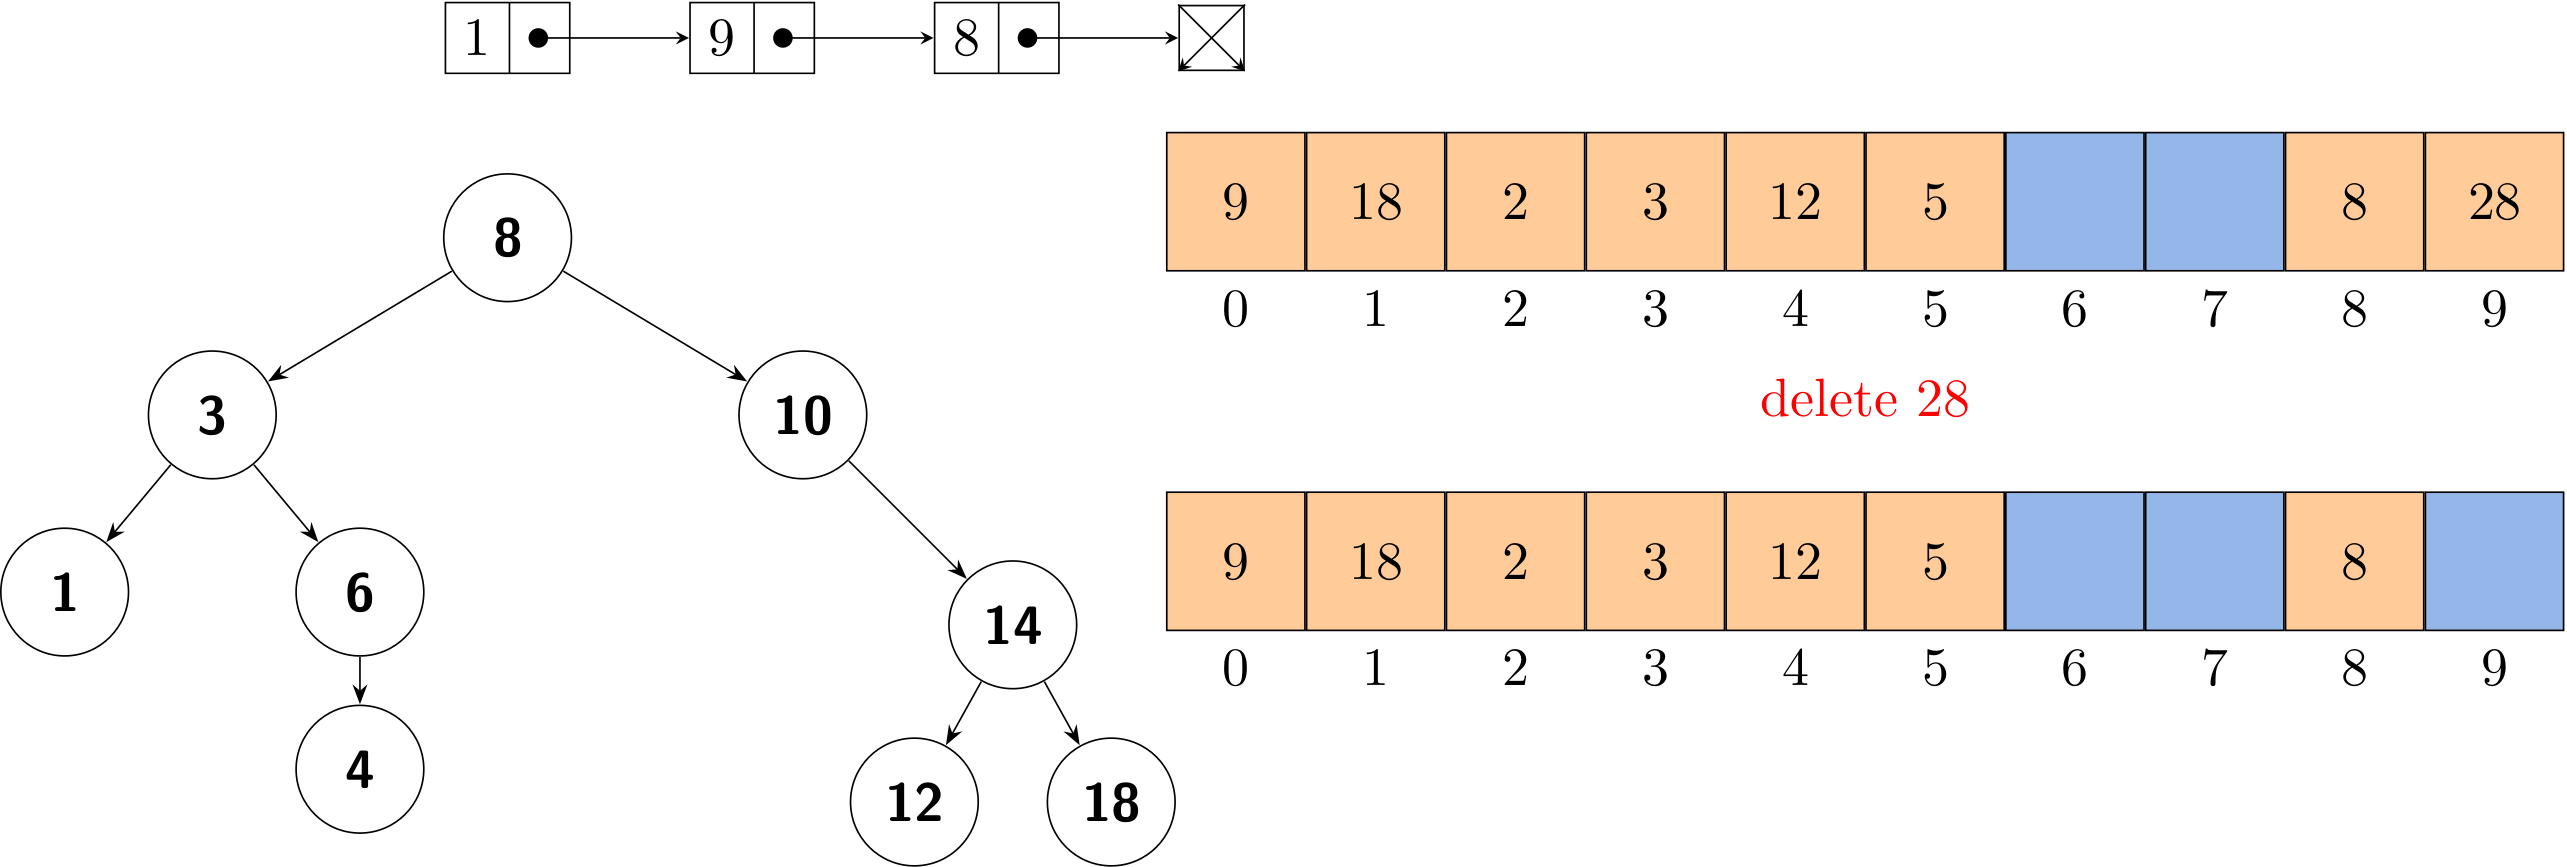
\includegraphics[height=0.6\paperheight]{cover}};
}
    \begin{frame}
        \section{\textcolor{darkmidnightblue}{1. Balanced Trees}}
    \end{frame}

}

\begin{frame}[fragile]
    \frametitle{1.1 What Is Balance?}

    \begin{columns}
        \column{.4\textwidth}
        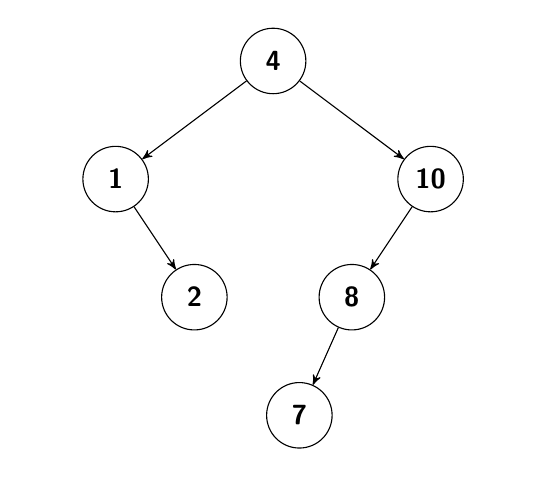
\begin{tikzpicture}[treenode/.style = {align=center, inner sep=1pt, text centered,
            font=\sffamily},
          bst/.style = {treenode, circle, black, font=\sffamily\bfseries, draw=black, text width=2em}, ->,>=stealth',level/.style={sibling distance = 4cm/#1,
          level distance = 1.5cm}]
        \node [bst] {4}
            child {node [bst] {1}
                child[edge from parent/.style={draw=none}] {node {}}
                child {node [bst](n6) {2}
                }
            }
            child {node (n10) [bst] {10}
               child {node [bst] {8}
                    child {node [bst] {7}}
                    child[edge from parent/.style={draw=none}] {node {}}
               }
               child[edge from parent/.style={draw=none}] {node {}}
            }
        ;
        \end{tikzpicture}
        \column{.59\textwidth}
       \faIcon{question-circle} Consider the following questions:
       
       \begin{itemize}
        \item Given a BST, what is time complexity of common operations (e.g., \texttt{search()}, \texttt{put()})?
        \item What is the height if inserting 1, 2, 4, 7, 8, and 10  sequentially?
       \end{itemize}
    \end{columns}

\end{frame}

\begin{frame}[fragile]

   \begin{columns}
    \column{.6\textwidth}
    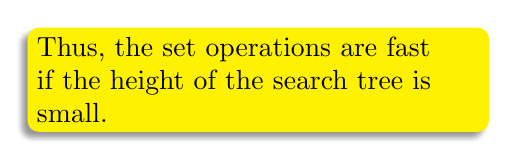
\begin{tikzpicture}
        \node[fill=yellow,blur shadow={shadow xshift=-0.5ex},
        text width=16em,anchor=south west,rounded corners]
        {Thus, the set operations
        are fast if the height of the search tree is small.};
    \end{tikzpicture}

    \begin{exampleblock}{Balanced Tree}
        A search tree is \alert{balanced} if it can guarantee that basic dynamic-set operations take $O(\lg{N})$ time in the worst case.
    \end{exampleblock} 
    \column{.39\textwidth}
    \begin{tikzpicture}[treenode/.style = {align=center, inner sep=.8pt, text centered,
        font=\sffamily},
      bst/.style = {treenode, circle, black, font=\sffamily\bfseries, draw=black, text width=1.8em}, ->,>=stealth',level/.style={sibling distance = 1.8cm,
      level distance = 1.2cm}]
    \node [bst] {1}
        child[edge from parent/.style={draw=none}] {node {}
        }
        child {node [bst] {2}
           child[edge from parent/.style={draw=none}] {node {}
           }
           child {node [bst] {4}
                child[edge from parent/.style={draw=none}] {node {}}
                child {node [bst] {7}
                   child[edge from parent/.style={draw=none}] {node {}}
                   child {node [bst] {8}
                     child[edge from parent/.style={draw=none}] {node {}
                       }
                     child {node [bst] {10}}
                   }
                }
           }
        }
    ;
    \end{tikzpicture}
\end{columns}

\end{frame}

\begin{frame}[fragile]
    \frametitle{1.2 Balanced Tree}
\begin{exampleblock}{Perfectly Height-balanced}
 A tree is \alert{perfectly} height-balanced if the left and right subtrees of any node are the same height.
\end{exampleblock}

\begin{columns}
    \column{.4\textwidth}<1->
    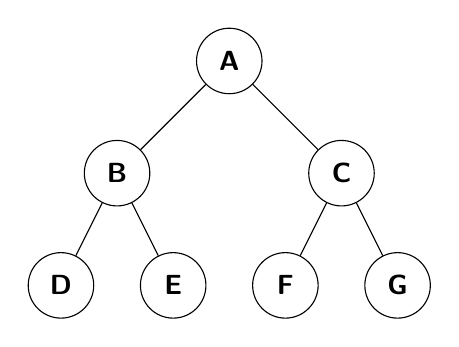
\begin{tikzpicture}[treenode/.style = {align=center, inner sep=1pt, text centered, font=\sffamily}, bst/.style = {treenode, circle, black, font=\sffamily\bfseries, draw=black, text width=2em},level/.style={sibling distance = 3cm/#1,
        level distance = 1.5cm}, scale=.95]
\node [bst] {A}
        child {node [bst] {B}
            child {node [bst] {D}}
            child {node [bst] {E}}
        }
        child {node [bst] {C}
            child {node [bst] {F}}
            child {node [bst] {G}}
        }
;
    \end{tikzpicture}     
    \column{.59\textwidth}<2->
    But \textbf{perfect height balance} is very rare: it is only possible if there are exactly $2^{H+1} - 1$ nodes.
\end{columns}

\end{frame}


\begin{frame}

    \section{\textcolor{darkmidnightblue}{2. AVL Tree}} 
    An AVL tree (named after inventors \textbf{A}delson-\textbf{V}elsky and \textbf{L}andis) is a self-balancing binary search tree (BST).
\end{frame}


\begin{frame}[fragile]
    \frametitle{2.1 AVL Definition}
\begin{block}{AVL Balance Property}
In an AVL tree, the heights of the two child subtrees of any node differ by \alert{at most one}.
\end{block}

\pause
\begin{columns}
    \column{.4\textwidth}
    \faIcon{question-circle} Is this an AVL tree?
    \column{.58\textwidth}
    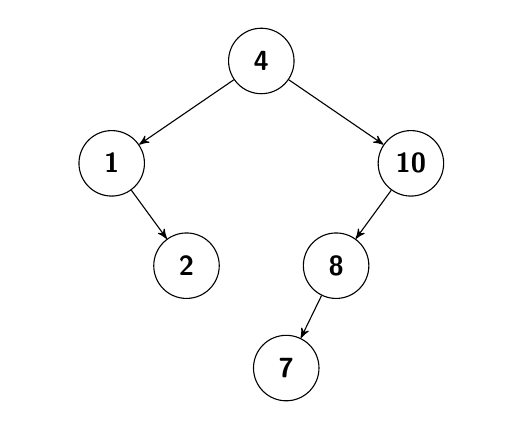
\begin{tikzpicture}[treenode/.style = {align=center, inner sep=1pt, text centered,
        font=\sffamily},
      bst/.style = {treenode, circle, black, font=\sffamily\bfseries, draw=black, text width=2em}, ->,>=stealth',level/.style={sibling distance = 3.8cm/#1,
      level distance = 1.3cm}]
    \node [bst] {4}
        child {node [bst] {1}
            child[edge from parent/.style={draw=none}] {node {}}
            child {node [bst](n6) {2}
            }
        }
        child {node (n10) [bst] {10}
           child {node [bst] {8}
                child {node [bst] {7}}
                child[edge from parent/.style={draw=none}] {node {}}
           }
           child[edge from parent/.style={draw=none}] {node {}}
        }
    ;
    \end{tikzpicture}
\end{columns}

\end{frame}

\begin{frame}
    \begin{lemma}
        An AVL tree with $n$ nodes has height $O(\lg{n})$. 
    \end{lemma}

    \begin{proof}
We use $N(h)$ to denote the minimum number of nodes in an AVL tree with height $h$. Then we have

\[
    N(h) \geq
\begin{cases}
    0,& h = -1\\
    1, & h = 0 \\
    1 + 2N(h - 2), & h \geq 1 \\
\end{cases}
\]

After $i$ steps, it is $N(h) \geq 1 + 2 + 4 + ... + 2^{i-1} + 2^iN(h-2i)$.
    \end{proof}
\end{frame}

\begin{frame}
\begin{proof}[Proof. (cont.)]
It can be simplified to
\[N(h) \geq 2^{i} - 1 + 2^iN(h-2i)\]

We solve $h-2i \leq 0$ to get the base case, giving $i = \frac{h}{2}$. Then we have
\[N(h) \geq 2^{h/2} - 1 + 2^{h/2}N(0) = 2^{h/2 + 1} - 1\] 

So we basically just got an inequality relating the number of nodes $n$ and the height $h$ of an AVL tree, $n\geq 2^{h/2 + 1} - 1$, which yields $h \leq 2\lg{(n + 1)} - 2$.
\end{proof}
    

\end{frame}

\begin{frame}
    \frametitle{Tight Bound of AVL Trees}
    The height $h$ of an AVL tree with $n$ nodes lies in the interval:

    \[ \log_{2}(n + 1) \leq h + 1 < \log_{\varphi}(n + 2) + b \]
where $\varphi = \frac{1 + \sqrt{5}}{2} \approx 1.618$, and $b \approx -0.3277$.
\end{frame}

\begin{frame}[fragile]
    \frametitle{2.2 Design of AVL Trees}
    
\faIcon{question-circle} To implement a node in an AVL trees, what else do we need based on a regular BST node?
    \begin{minted}[bgcolor=LightGray]{python}
class Node:
    def __init__(self, key, left=None, right=None):
        self.key = key
        self.left = left
        self.right = right
    \end{minted}
\end{frame}

\begin{frame}[fragile]

\begin{minted}[bgcolor=LightGray, baselinestretch=1.1]{python}
class Node:
    def __init__(self, key, height=0, 
                 left=None, right=None):
        self.key = key
        self.height = height
        self.left = left
        self.right = right

class AVL:
    def __init__(self):
        self.root = None
\end{minted}
\faIcon{pen} How to get the height of an AVL tree?
\end{frame}

\begin{frame}
    \frametitle{Balance Factor}
We can introduce \alert{balance factor} $BF(x)$ of node $x$, which is defined to be the height difference of its two child subtrees 

\[BF(x) = h(x.left) - h(x.right)\]

According to the \textbf{AVL balance property}, $BF(x) \in \underline{\hspace{3cm}}$.

\end{frame}

\begin{frame}[fragile]
    \frametitle{2.3 \texttt{get()} in AVL Trees}

It works exactly in the same way a BST does.

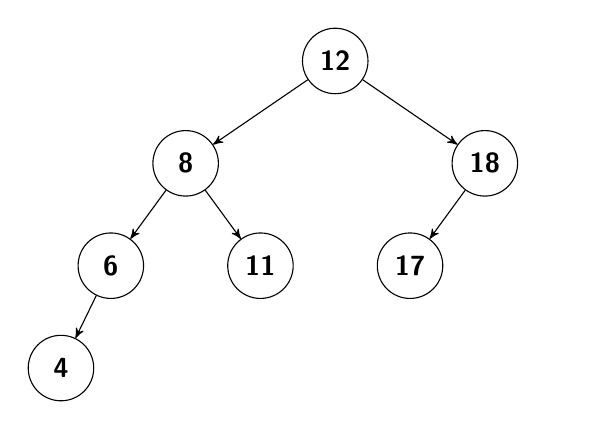
\begin{tikzpicture}[treenode/.style = {align=center, inner sep=1pt, text centered,
    font=\sffamily},
  bst/.style = {treenode, circle, black, font=\sffamily\bfseries, draw=black, text width=2em}, ->,>=stealth',level/.style={sibling distance = 3.8cm/#1,
  level distance = 1.3cm}]
\node [bst] {12}
    child {node [bst] {8}
        child {node [bst] {6}
            child {node [bst] {4}}
            child[edge from parent/.style={draw=none}] {node {}}
        }
        child {node [bst] {11}
        }
    }
    child {node [bst] {18}
       child {node [bst] {17}}
       child[edge from parent/.style={draw=none}] {node {}}
    }
;
\end{tikzpicture}
    
\end{frame}

\begin{frame}[fragile]

\begin{minted}[bgcolor=LightGray,]{python}
def get(self, key):
    def _get(x: Node):
        if x is None or key == x.key:
            return x
        if key < x.key:
            return _get(x.left)
        else:
            return _get(x.right)
    if key is None:
        raise KeyError
    return _get(self._root)
\end{minted}

\end{frame}

\begin{frame}[fragile]
    \frametitle{2.4 \texttt{put()} in AVL Trees}
\faIcon{lightbulb} What happens if we insert 1 into the AVL tree?

\begin{columns}
    \column{.49\textwidth}<1->
    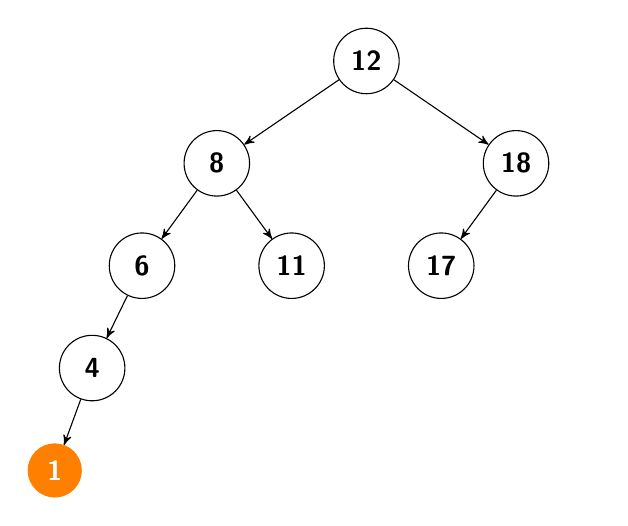
\begin{tikzpicture}[treenode/.style = {align=center, inner sep=1pt, text centered,
        font=\sffamily},
      bst/.style = {treenode, circle, black, font=\sffamily\bfseries, draw=black, text width=2em}, orangebst/.style = {treenode, circle, white, font=\sffamily\bfseries, draw=orange, fill=orange, text width=1.5em}, ->,>=stealth',level/.style={sibling distance = 3.8cm/#1,
      level distance = 1.3cm}]
    \node [bst] {12}
        child {node [bst] {8}
            child {node [bst] {6}
                child {node [bst] {4}
                    child {node [orangebst] {1}}
                    child[edge from parent/.style={draw=none}] {node {}}
                }
                child[edge from parent/.style={draw=none}] {node {}}
            }
            child {node [bst] {11}
            }
        }
        child {node [bst] {18}
           child {node [bst] {17}}
           child[edge from parent/.style={draw=none}] {node {}}
        }
    ;
    \end{tikzpicture}    
    \column{.6\textwidth}<2-> 
    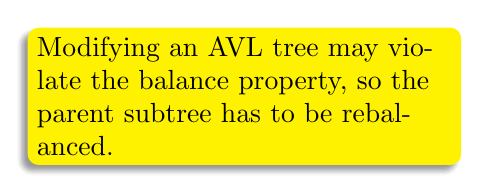
\begin{tikzpicture}
        \node[fill=yellow,blur shadow={shadow xshift=-0.5ex},
        text width=15em,anchor=south west,rounded corners]
        {Modifying an AVL tree may violate the balance property, so the parent subtree has to be \alert{rebalanced}.};
    \end{tikzpicture}
    \begin{enumerate}
        \item Insert the key in the same way a BST does.
        \item Re-balance.
    \end{enumerate}
\end{columns}

\end{frame}

{\setbeamercolor{palette primary}{fg=black, bg=yellow}
\begin{frame}[standout]
  Re-balance an AVL is mainly based on \alert{tree rotations} on a BST.
\end{frame}
}

\begin{frame}[fragile]
    \frametitle{2.5 Rotations}
There are two kinds of rotations: left rotations and right rotations.
    
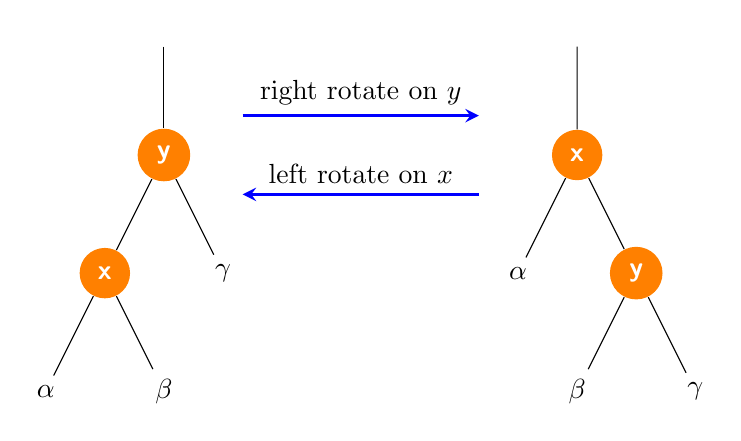
\begin{tikzpicture}[bnode/.style = {align=center, inner sep=1pt, text centered, circle, white, font=\sffamily\bfseries, 
    fill=orange, text width=1.5em},]
    \node (lefttree) {}
        child { node [bnode] {y}
            child {node [bnode] {x}
                child {node {$\alpha$}}
                child {node {$\beta$}}
            }
            child {node {$\gamma$}}
            };
    
    \draw [-stealth, line width=0.4mm, draw=blue](1,-1) -- (4,-1)node[midway,above,shape=rectangle,draw=none]{right rotate on $y$};

    \draw [stealth-, line width=0.4mm, draw=blue](1,-2) -- (4,-2)node[midway,above,shape=rectangle,draw=none]{left rotate on $x$}; 

    \node (right) [right=5cm of lefttree] {}
            child { node [bnode] {x}
                child {node {$\alpha$}}
                child {node [bnode] {y}
                    child {node {$\beta$}}
                    child {node {$\gamma$}}
                    }
    };
\end{tikzpicture}

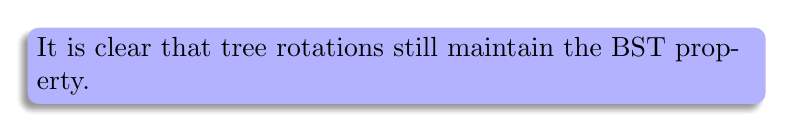
\begin{tikzpicture}
    \node[fill=blue!30,blur shadow={shadow xshift=-0.5ex},
    text width=26em,anchor=south west,rounded corners]
    {It is clear that tree rotations still maintain the BST property.};
\end{tikzpicture}
\end{frame}

\begin{frame}
    \frametitle{Right Rotation}
\scalebox{.9}{
    \begin{algorithm}[H]
        \caption{right-rotate(y)}
        \KwIn{A node $y$ of an AVL tree}
        \KwOut{The new root after a right rotation}
        $x\gets y.left$ \\
        $y.left\gets x.right$ \\
        $x.right\gets y$ \\
        \tcp{Update height (only for AVL trees)}
        $y.height\gets max(h(y.left), h(y.right)) + 1$ \\
        $x.height\gets max(h(x.left), h(x.right)) + 1$ \\
        \Return{x}
    \end{algorithm}
}
\end{frame}

\begin{frame}
    \frametitle{Left Rotation}

\scalebox{.9}{
    \begin{algorithm}[H]
        \caption{left-rotate(x)}
        \KwIn{A node $y$ of an AVL tree}
        \KwOut{The new root after a left rotation}
        $y\gets x.right$ \\
        $x.right\gets y.left$ \\
        $y.left\gets x$ \\
        \tcp{Update height (only for AVL trees)}
        $x.height\gets max(h(x.left), h(x.right)) + 1$ \\
        $y.height\gets max(h(y.left), h(y.right)) + 1$ \\
        \Return{y}
    \end{algorithm}
}

\end{frame}

\begin{frame}[fragile]
    \frametitle{2.6 Re-balance}
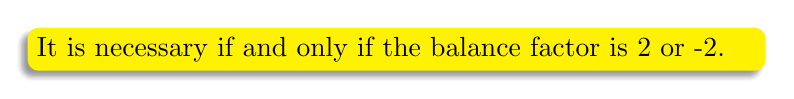
\begin{tikzpicture}
    \node[fill=yellow,blur shadow={shadow xshift=-0.5ex},
    text width=26em,anchor=south west,rounded corners]
    {It is necessary if and only if the \alert{balance factor} is 2 or -2.};
\end{tikzpicture}

\textbf{Case 1 (left-left)}: If $bf(x) = 2$ and $key < x.left.key$, then we make a right-rotation on $x$.

\begin{tikzpicture}[treenode/.style = {align=center, inner sep=1pt, text centered,
    font=\sffamily},
  bst/.style = {treenode, circle, black, font=\sffamily\bfseries, draw=black, text width=2em}, orangebst/.style = {treenode, circle, white, font=\sffamily\bfseries, draw=orange, fill=orange, text width=1.5em}, ->,>=stealth',level/.style={sibling distance = 3.8cm/#1,
  level distance = 1.3cm}]
  \node (lefttree) {}
    child {node [bst] {x}
       child {node [bst] {y}
         child {node[red] {$\alpha$}}
         child {node {$\beta$}}
       }
       child {node {$\gamma$}}
    }
  ;
    \draw [-stealth, line width=0.4mm, draw=blue](2.5,-2) -- (4.5,-2)node[midway,above,shape=rectangle,draw=none]{right rotate};

    \node [right=of lefttree, xshift=6cm] {}
        child {node [bst] {y}
            child {node [red] {$\alpha$}}
            child {node [bst] {x}
                child {node {$\beta$}}
                child {node {$\gamma$}}
            }
        }
    ;
\end{tikzpicture}

\end{frame}

\begin{frame}[fragile]

    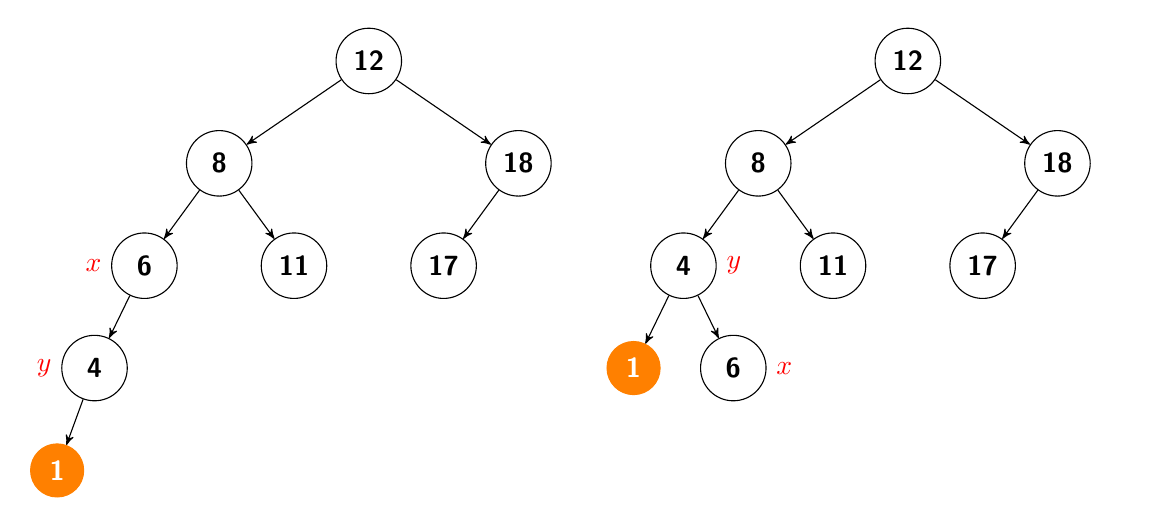
\begin{tikzpicture}[treenode/.style = {align=center, inner sep=1pt, text centered,
        font=\sffamily},
      bst/.style = {treenode, circle, black, font=\sffamily\bfseries, draw=black, text width=2em}, orangebst/.style = {treenode, circle, white, font=\sffamily\bfseries, draw=orange, fill=orange, text width=1.5em}, ->,>=stealth',level/.style={sibling distance = 3.8cm/#1,
      level distance = 1.3cm}]
    \node (lefttree) [bst] {12}
        child {node [bst] {8}
            child {node [bst](1n6) {6}
                child {node [bst](1n4) {4}
                    child {node [orangebst] {1}}
                    child[edge from parent/.style={draw=none}] {node {}}
                }
                child[edge from parent/.style={draw=none}] {node {}}
            }
            child {node [bst] {11}
            }
        }
        child {node [bst] {18}
           child {node [bst] {17}}
           child[edge from parent/.style={draw=none}] {node {}}
        }
    ;
    \node[left, red] at (1n6.west) {$x$};
    \node[left, red] at (1n4.west){$y$};

    \node [bst, right=of lefttree, xshift=5cm] {12}
    child {node [bst] {8}
        child {node [bst](2n4) {4}
            child {node [orangebst] {1}
            }
            child {node [bst](2n6) {6}}
        }
        child {node [bst] {11}
        }
    }
    child {node [bst] {18}
       child {node [bst] {17}}
       child[edge from parent/.style={draw=none}] {node {}}
    }
;
\node[right, red] at (2n6.east) {$x$};
\node[right, red] at (2n4.east) {$y$};
    \end{tikzpicture}  
\pause

\faIcon{lightbulb} Please prove that a right rotation can re-balance Case 1.
\end{frame}

\begin{frame}[fragile]
    \frametitle{Case 2}
\textbf{Case 2 (right-right)}: If $bf(x) = -2$ and $key > x.right.key$, then we make left-rotation on $x$.

\begin{tikzpicture}[treenode/.style = {align=center, inner sep=1pt, text centered,
    font=\sffamily},
  bst/.style = {treenode, circle, black, font=\sffamily\bfseries, draw=black, text width=2em}, orangebst/.style = {treenode, circle, white, font=\sffamily\bfseries, draw=orange, fill=orange, text width=1.5em}, ->,>=stealth',level/.style={sibling distance = 3.8cm/#1,
  level distance = 1.3cm}]
\node (lefttree) {}
    child {node [bst] {x}
        child {node {$\alpha$}}
        child {node [bst] {y}
            child {node {$\beta$}}
            child {node [red] {$\gamma$}}
        }
    }
;

\draw [-stealth, line width=0.4mm, draw=blue](2.5,-2) -- (4.5,-2)node[midway,above,shape=rectangle,draw=none]{left rotate};

\node [right=of lefttree, xshift=6cm] {}
    child {node [bst] {y}
        child {node [bst] {x}
            child {node {$\alpha$}}
            child {node {$\beta$}}
        }
        child {node [red] {$\gamma$}}
    }
;

\end{tikzpicture}

\end{frame}

\begin{frame}[fragile]
    \frametitle{Case 3}
\textbf{Case 3 (left-right)}: If $bf(x) = 2$ and $key > x.left.key$, then we make a left rotation on $x.left$, and then make a right rotation on $x$.
    
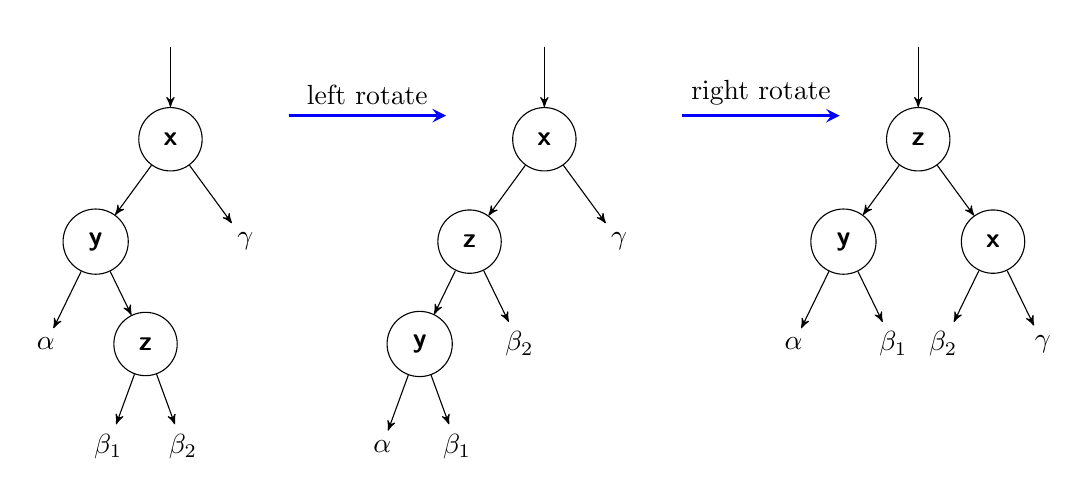
\begin{tikzpicture}[treenode/.style = {align=center, inner sep=1pt, text centered,
    font=\sffamily},
  bst/.style = {treenode, circle, black, font=\sffamily\bfseries, draw=black, text width=2em}, orangebst/.style = {treenode, circle, white, font=\sffamily\bfseries, draw=orange, fill=orange, text width=1.5em}, ->,>=stealth',level/.style={sibling distance = 3.8cm/#1,
  level distance = 1.3cm}]
\node (lefttree) {}
    child {node [bst] {x}
        child {node [bst] {y}
            child {node {$\alpha$}}
            child {node [bst] {z}
                child {node {$\beta_1$}}
                child {node {$\beta_2$}}
            }
        }
        child {node {$\gamma$}}
    }
;

\draw [-stealth, line width=0.4mm, draw=blue](1.5,-1) -- (3.5,-1)node[midway,above,shape=rectangle,draw=none]{left rotate};

\node (midtree) [right=of lefttree, xshift=3.5cm] {}
    child {node [bst] {x}
        child {node [bst] {z}
            child {node [bst] {y}
                child {node {$\alpha$}}
                child {node {$\beta_1$}}
            }
            child {node {$\beta_2$}}
        }
        child {node {$\gamma$}}
    }
;

\draw [-stealth, line width=0.4mm, draw=blue](6.5,-1) -- (8.5,-1)node[midway,above,shape=rectangle,draw=none]{right rotate};

\node (righttree) [right=of midtree, xshift=3.5cm] {}
    child {node [bst] {z}
        child {node [bst] {y}
                child {node {$\alpha$}}
                child {node {$\beta_1$}}
            }
        child {node [bst] {x}
            child {node {$\beta_2$}}
            child {node {$\gamma$}}
        }
    }
;
\end{tikzpicture}
\end{frame}

\begin{frame}[fragile]
    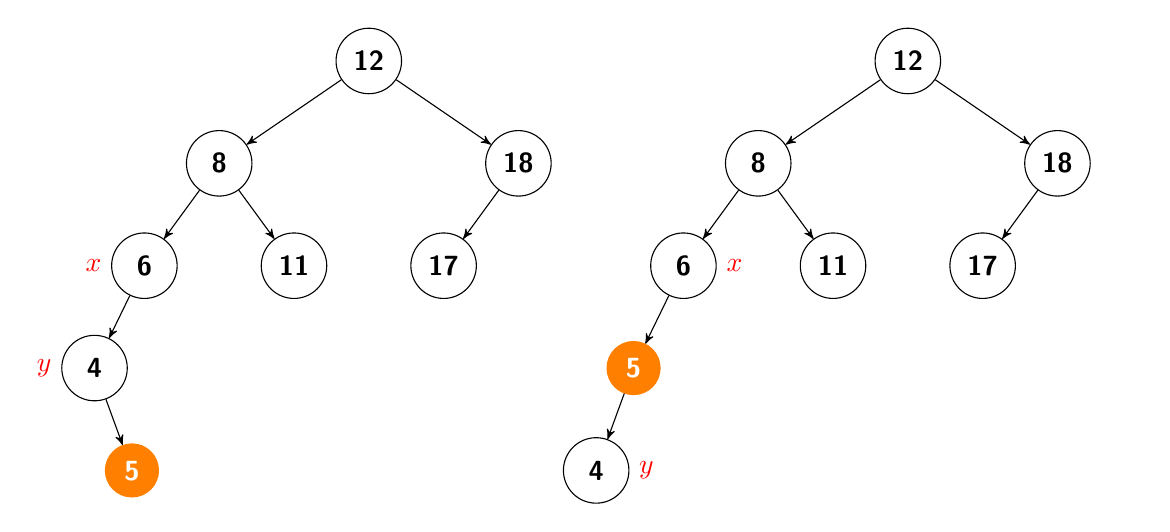
\begin{tikzpicture}[treenode/.style = {align=center, inner sep=1pt, text centered,
        font=\sffamily},
      bst/.style = {treenode, circle, black, font=\sffamily\bfseries, draw=black, text width=2em}, orangebst/.style = {treenode, circle, white, font=\sffamily\bfseries, draw=orange, fill=orange, text width=1.5em}, ->,>=stealth',level/.style={sibling distance = 3.8cm/#1,
      level distance = 1.3cm},]
    \node (lefttree) [bst] {12}
        child {node [bst] {8}
            child {node [bst](1n6) {6}
                child {node [bst](1n4) {4}
                 child[edge from parent/.style={draw=none}] {node {}}
                 child {node [orangebst] {5}}
                }
                child[edge from parent/.style={draw=none}] {node {}}
            }
            child {node [bst] {11}
            }
        }
        child {node [bst] {18}
           child {node [bst] {17}}
           child[edge from parent/.style={draw=none}] {node {}}
        }
    ;
    \node[left, red] at (1n6.west) {$x$};
    \node[left, red] at (1n4.west){$y$};

    \node [bst, right=of lefttree, xshift=5cm] {12}
    child {node [bst] {8}
        child {node [bst](2n6) {6}
            child {node [orangebst] {5}
              child {node [bst](2n4) {4}}
              child[edge from parent/.style={draw=none}] {node {}}
            }
            child[edge from parent/.style={draw=none}] {node {}}
        }
        child {node [bst] {11}
        }
    }
    child {node [bst] {18}
       child {node [bst] {17}}
       child[edge from parent/.style={draw=none}] {node {}}
    }
;
\node[right, red] at (2n6.east) {$x$};
\node[right, red] at (2n4.east) {$y$};
    \end{tikzpicture}  
    
    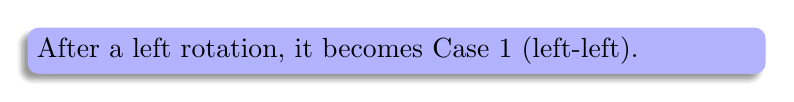
\begin{tikzpicture}
        \node[fill=blue!30,blur shadow={shadow xshift=-0.5ex},
        text width=26em,anchor=south west,rounded corners]
        {After a left rotation, it becomes Case 1 (left-left).};
    \end{tikzpicture}

\end{frame}

\begin{frame}[fragile]

    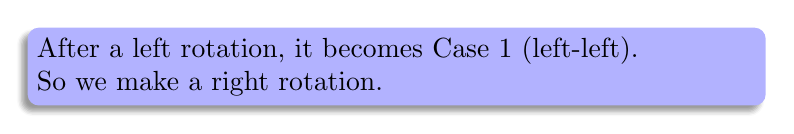
\begin{tikzpicture}
        \node[fill=blue!30,blur shadow={shadow xshift=-0.5ex},
        text width=26em,anchor=south west,rounded corners]
        {After a left rotation, it becomes Case 1 (left-left). 
        
        So we make a right rotation.};
    \end{tikzpicture}

    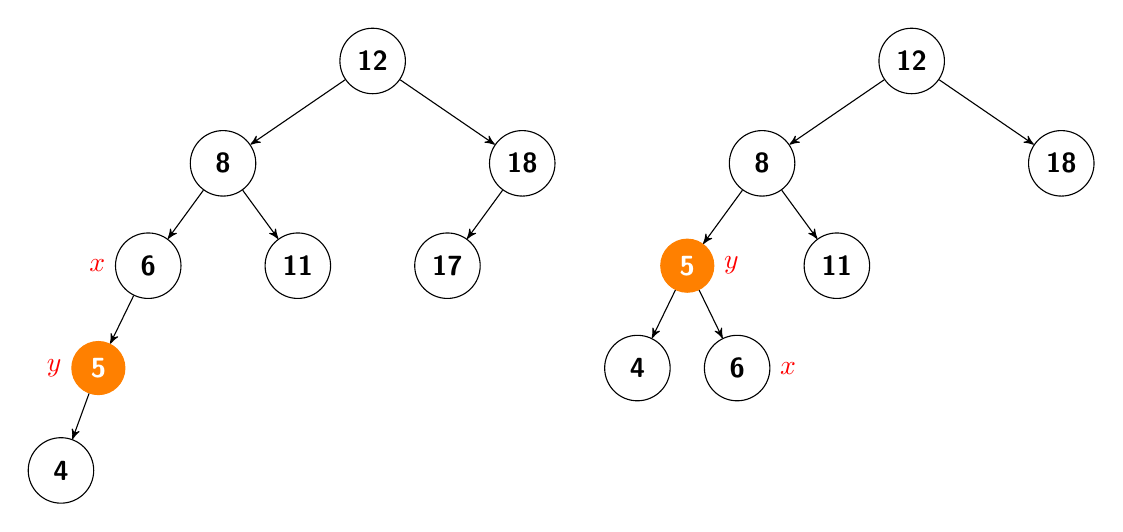
\begin{tikzpicture}[treenode/.style = {align=center, inner sep=1pt, text centered,
        font=\sffamily},
      bst/.style = {treenode, circle, black, font=\sffamily\bfseries, draw=black, text width=2em}, orangebst/.style = {treenode, circle, white, font=\sffamily\bfseries, draw=orange, fill=orange, text width=1.5em}, ->,>=stealth',level/.style={sibling distance = 3.8cm/#1,
      level distance = 1.3cm},]

    \node [bst](lefttree) {12}
    child {node [bst] {8}
        child {node [bst](1n6) {6}
            child {node [orangebst](1n5) {5}
              child {node [bst] {4}}
              child[edge from parent/.style={draw=none}] {node {}}
            }
            child[edge from parent/.style={draw=none}] {node {}}
        }
        child {node [bst] {11}
        }
    }
    child {node [bst] {18}
       child {node [bst] {17}}
       child[edge from parent/.style={draw=none}] {node {}}
    }
;
\node[left, red] at (1n6.west) {$x$};
\node[left, red] at (1n5.west) {$y$};

\node [bst, right=of lefttree, xshift=5cm] {12}
    child {node [bst] {8}
        child {node [orangebst](2n5) {5}
            child {node [bst] {4}}
            child {node [bst](2n6) {6}}
        }
        child {node [bst] {11}}
    }
    child {node [bst] {18}}
;

\node[right, red] at (2n6.east) {$x$};
\node[right, red] at (2n5.east) {$y$};
    \end{tikzpicture}  

\end{frame}

\begin{frame}[fragile]
    \frametitle{Case 4}
\textbf{Case 4 (right-left)}: If $bf(x) = -2$ and $key < x.right.key$, then we make a right rotation on $x.right$, and make a left rotation on $x$.

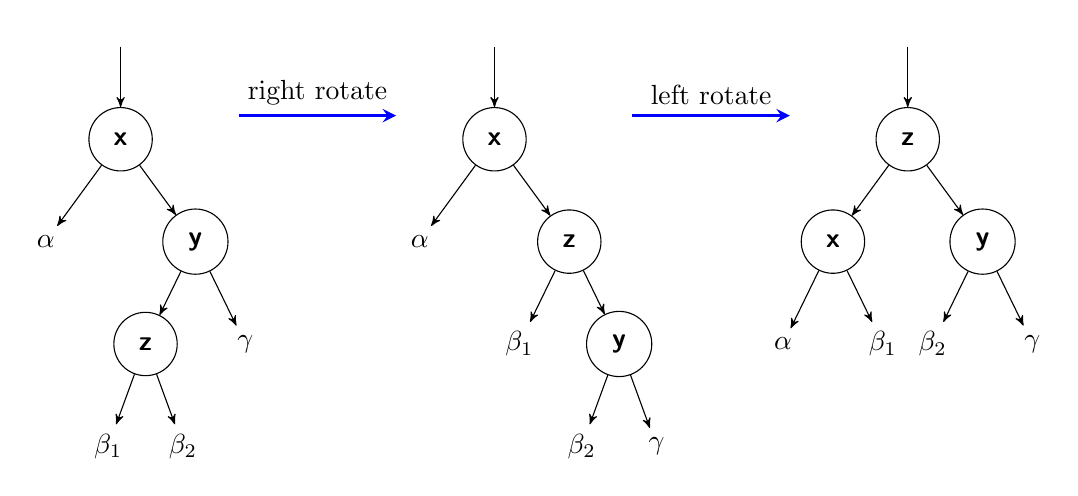
\begin{tikzpicture}[treenode/.style = {align=center, inner sep=1pt, text centered,
    font=\sffamily},
  bst/.style = {treenode, circle, black, font=\sffamily\bfseries, draw=black, text width=2em}, orangebst/.style = {treenode, circle, white, font=\sffamily\bfseries, draw=orange, fill=orange, text width=1.5em}, ->,>=stealth',level/.style={sibling distance = 3.8cm/#1,
  level distance = 1.3cm}]
\node (lefttree) {}
    child {node [bst] {x}
        child {node {$\alpha$}}
        child {node [bst] {y}
            child {node [bst] {z}
                child {node {$\beta_1$}}
                child {node {$\beta_2$}}
            }
            child {node {$\gamma$}}
        }
    }
;

\draw [-stealth, line width=0.4mm, draw=blue](1.5,-1) -- (3.5,-1)node[midway,above,shape=rectangle,draw=none]{right rotate};

\node [right=of lefttree, xshift=3.5cm] (midtree) {}
    child {node [bst] {x}
        child {node {$\alpha$}}
        child {node [bst] {z}
            child {node {$\beta_1$}
            }
            child {node [bst] {y}
                child {node {$\beta_2$}}
                child {node {$\gamma$}}
            }
        }
    }
;

\draw [-stealth, line width=0.4mm, draw=blue](6.5,-1) -- (8.5,-1)node[midway,above,shape=rectangle,draw=none]{left rotate};

\node [right=of midtree, xshift=4cm] {}
   child {node [bst] {z}
    child {node [bst] {x}
        child {node {$\alpha$}}
        child {node {$\beta_1$}}
    }
    child {node [bst] {y}
     child {node {$\beta_2$}}
     child {node {$\gamma$}}
    }
   }
;

\end{tikzpicture}

\end{frame}

\begin{frame}[fragile]
    \frametitle{2.7 Complete \texttt{put()}}

    \begin{minted}[bgcolor=LightGray, baselinestretch=1]{python}
def put(self, key):
    def _put(x: AVL.Node):
        # step 1: regular BST insert (TO DO)
        # step 2: update the height
        x.height = max(AVL._get_height(x.left), 
                       AVL._get_height(x.right)) + 1
        # step 3: get the balance factor
        bf = AVL._get_balance_factor(x)
        # step 4: re-balance (TO DO)
        return x
    self._root = _put(self._root)
    \end{minted}
\end{frame}

\begin{frame}[fragile]
    \frametitle{Step 1}
    \begin{minted}[bgcolor=LightGray,]{python}
# step 1: regular BST insert
if x is None:
    return AVL.Node(key)
elif key < x.key:
    x.left = _put(x.left)
elif key > x.key:
    x.right = _put(x.right)
    \end{minted}

\end{frame}

\begin{frame}[fragile]
    \frametitle{Step 4}
\begin{minted}[bgcolor=LightGray]{python}
if bf > 1 and key < x.left.key:  # case 1
    return AVL._right_rotate(x)
if bf < -1 and key > x.right.key:  # case 2
    return AVL._left_rotate(x)
if bf > 1 and key > x.left.key:  # case 3
    x.left = AVL._left_rotate(x.left)
    return AVL._right_rotate(x)
if bf < -1 and key < x.right.key:  # case 4
    x.right = AVL._right_rotate(x.right)
    return AVL._left_rotate(x)    
\end{minted}
    

\end{frame}

\begin{frame}[fragile]
    \frametitle{2.8 \texttt{remove()} in AVL Trees}

    \faIcon{lightbulb} What happens if we delete 11 from the AVL tree?

    \begin{columns}
        \column{.4\textwidth}<1->
        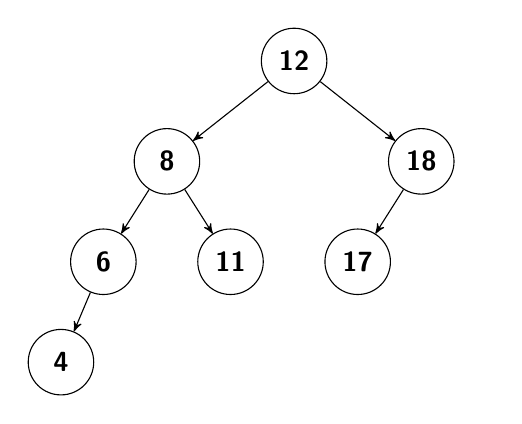
\begin{tikzpicture}[treenode/.style = {align=center, inner sep=1pt, text centered,
            font=\sffamily},
          bst/.style = {treenode, circle, black, font=\sffamily\bfseries, draw=black, text width=2em}, orangebst/.style = {treenode, circle, white, font=\sffamily\bfseries, draw=orange, fill=orange, text width=1.5em}, ->,>=stealth',level/.style={sibling distance = 3.8cm/#1,
          level distance = 1.5cm}, scale=.85]
        \node [bst] {12}
            child {node [bst] {8}
                child {node [bst] {6}
                    child {node [bst] {4}
                    }
                    child[edge from parent/.style={draw=none}] {node {}}
                }
                child {node [bst] {11}
                }
            }
            child {node [bst] {18}
               child {node [bst] {17}}
               child[edge from parent/.style={draw=none}] {node {}}
            }
        ;
        \end{tikzpicture}    
        \column{.6\textwidth}<2-> 
        \scalebox{.9}{
            \begin{algorithm}[H]
                \caption{remove(x, key)}
                \tcp{step 1: regular BST delete (TO DO)}
                \tcp{step 2: update the height}
                $x.height\gets max(h(x.left), h(x.right)) + 1$ \\
                \tcp{step 3: get the balance factor}
                $bf\gets bf(x)$ \\
                \tcp{step 4: re-balance (TO DO)}
                \Return{x}
            \end{algorithm}
        }
    \end{columns}
    
\end{frame}

\begin{frame}
    \frametitle{Review \texttt{remove()} on a BST}
\scalebox{.7}{
    \begin{algorithm}[H]
        \caption{remove(x, key)}
        \begin{multicols}{2}
            \If{x == null}{
                \Return{null}
            }
            \uIf{key $<$ x.key}{
                $x.left\gets remove(x.left, key)$
            }\uElseIf{key $>$ x.key}{
                $x.right\gets remove(x.right, key)$
            }\Else{
                \If{x.right == null}{
                    \Return{x.left}
                }
                \If{x.left == null}{
                    \Return{x.right}
                }
                $t\gets x$ \\
                $x\gets min(t.right)$ \\
                $x.right\gets removeMin(t.right)$ \\
                $x.left\gets t.left$
            }
            \Return{x}
        \end{multicols}
        \end{algorithm}
}
\end{frame}

\begin{frame}[fragile]
    \frametitle{Step 4}
    \begin{minted}[bgcolor=LightGray]{python}
if bf > 1 and AVL._get_balance_factor(x.left) >= 0:
    return AVL._right_rotate(x) # case 1: left-left
if bf < -1 and AVL._get_balance_factor(x.right) <= 0:
    return AVL._left_rotate(x)  # case 2: right-right
if bf > 1 and AVL._get_balance_factor(x.left) < 0:
    x.left = AVL._left_rotate(x.left)
    return AVL._right_rotate(x)  # case 3: left-right
if bf < -1 and AVL._get_balance_factor(x.right) > 0:
    x.right = AVL._right_rotate(x.right)
    return AVL._left_rotate(x)  # case 4: right-left
    \end{minted}

\end{frame}

% \begin{frame}[fragile]

% \begin{tikzpicture}
%     \node[fill=yellow,blur shadow={shadow xshift=-0.5ex},
%     text width=26em,anchor=south west,rounded corners]
%     {It is feasible to store the \texttt{height} within each node, but it is not necessary to know the absolute height. };
% \end{tikzpicture}

% \pause
% We can introduce \alert{balance factor} $BF(x)$ of node $x$, which is defined to be the height difference of its two child subtrees (i.e., $BF(x) = h(x.right) - h(x.left)$).

% According to the \textbf{AVL balance property}, $BF(x) \in \underline{\hspace{3cm}}$.

% \begin{minted}[bgcolor=LightGray, fontsize=\small]{python}
% class Node:
%     def __init__(self, key, bf=0, left=None, right=None):
%         self.key = key
%         self.bf = bf
%         self.left = left
%         self.right = right
% \end{minted}

% \end{frame}

% \begin{frame}[fragile]
%     \frametitle{2.3 \texttt{get()} in AVL Trees}
% It works exactly in the same way a BST does.

% \begin{tikzpicture}[treenode/.style = {align=center, inner sep=1pt, text centered,
%     font=\sffamily},
%   bst/.style = {treenode, circle, black, font=\sffamily\bfseries, draw=black, text width=2em}, ->,>=stealth',level/.style={sibling distance = 3.8cm/#1,
%   level distance = 1.3cm}]
% \node [bst] {12}
%     child {node [bst] {8}
%         child {node [bst] {5}
%             child {node [bst] {4}}
%             child[edge from parent/.style={draw=none}] {node {}}
%         }
%         child {node [bst] {11}
%         }
%     }
%     child {node [bst] {18}
%        child {node [bst] {17}}
%        child[edge from parent/.style={draw=none}] {node {}}
%     }
% ;
% \end{tikzpicture}

% \end{frame}

% \begin{frame}[fragile]

% \begin{minted}[bgcolor=LightGray,]{python}
% def get(self, key):
%     def _get(x: AVL.Node):
%         if x is None or key == x.key:
%             return x
%         if key < x.key:
%             return _get(x.left)
%         else:
%             return _get(x.right)
%     if key is None:
%         raise KeyError
%     return _get(self._root)
% \end{minted}

% \end{frame}

% \begin{frame}[fragile]
%     \frametitle{2.4 \texttt{put()} in AVL Trees}
% \faIcon{lightbulb} What happens if we insert 1 into the AVL tree?

% \begin{columns}
%     \column{.49\textwidth}<1->
%     \begin{tikzpicture}[treenode/.style = {align=center, inner sep=1pt, text centered,
%         font=\sffamily},
%       bst/.style = {treenode, circle, black, font=\sffamily\bfseries, draw=black, text width=2em}, orangebst/.style = {treenode, circle, white, font=\sffamily\bfseries, draw=orange, fill=orange, text width=1.5em}, ->,>=stealth',level/.style={sibling distance = 3.8cm/#1,
%       level distance = 1.3cm}]
%     \node [bst] {12}
%         child {node [bst] {8}
%             child {node [bst] {5}
%                 child {node [bst] {4}
%                     child {node [orangebst] {1}}
%                     child[edge from parent/.style={draw=none}] {node {}}
%                 }
%                 child[edge from parent/.style={draw=none}] {node {}}
%             }
%             child {node [bst] {11}
%             }
%         }
%         child {node [bst] {18}
%            child {node [bst] {17}}
%            child[edge from parent/.style={draw=none}] {node {}}
%         }
%     ;
%     \end{tikzpicture}    
%     \column{.6\textwidth}<2-> 
%     \begin{tikzpicture}
%         \node[fill=yellow,blur shadow={shadow xshift=-0.5ex},
%         text width=15em,anchor=south west,rounded corners]
%         {Modifying an AVL tree may violate the balance property, so the parent subtree has to be \alert{rebalanced}.};
%     \end{tikzpicture}
%     \begin{enumerate}
%         \item Insert the key in the same way a BST does.
%         \item Re-balance.
%     \end{enumerate}
% \end{columns}

% \end{frame}

% \begin{frame}[fragile]
% If the node maintains the \alert{\texttt{parent}} link, the implementation will be easier to understand.
    
% \begin{tikzpicture}[treenode/.style = {align=center, inner sep=1pt, text centered,
%     font=\sffamily},
%   bst/.style = {treenode, circle, black, font=\sffamily\bfseries, draw=black, text width=2em}, orangebst/.style = {treenode, circle, white, font=\sffamily\bfseries, draw=orange, fill=orange, text width=1.5em}, ->,>=stealth',level/.style={sibling distance = 3.8cm/#1,
%   level distance = 1.3cm}]
% \node [bst](lefttree) {12}
%     child {node [bst] {8}
%         child {node [bst](n5) {5}
%             child {node [bst](n4) {4}
%                 child {node [orangebst](n1) {1}}
%                 child[edge from parent/.style={draw=none}] {node {}}
%             }
%             child[edge from parent/.style={draw=none}] {node {}}
%         }
%         child {node [bst] {11}
%         }
%     }
%     child {node [bst] {18}
%        child {node [bst] {17}}
%        child[edge from parent/.style={draw=none}] {node {}}
%     }
% ;
% \node[right] at (n1.east) {$z$};
% \node[right] at (n4.east) {$z.p$};
% \node[left] at (n5.west) {$z.p.p$};

% \draw [-stealth, line width=0.6mm, draw=blue](2.5,0) -- (4.5,0){};

% \node [bst, right=of lefttree, xshift=5cm] {12}
% child {node [bst] {8}
% child {node [bst] {4}
%     child {node [bst] {1}
%     }
%     child {node [bst] {5}}
% }
% child {node [bst] {11}
% }
% }
% child {node [bst] {18}
% child {node [bst] {17}}
% child[edge from parent/.style={draw=none}] {node {}}
% }
% ;
% \end{tikzpicture}   

% \end{frame}

% \begin{frame}[fragile]
%    \scalebox{.9}{
%     \begin{algorithm}[H]
%         \caption{put(key)}
%         \KwIn{A new $key$}
%         \begin{multicols}{2}
%             $z\gets Node(key)$ \\
%             $x\gets root$ \\
%             $y\gets null$ \\
%             \While{x $\neq$ null}{
%                 $y\gets x$ \\
%                 \uIf{key $<$ x.key}{
%                     $x\gets x.left$
%                 }\uElseIf{key $>$ x.key} {
%                     $x\gets x.right$
%                 }\uElse{
%                     \Return{} 
%                 }
%             }
%             \tcp{end of while}
%             $z.p\gets y$ \\
%             \uIf{y = null}{
%                 $root\gets z$ 
%             }\uElseIf{z.key $<$ y.key}{
%                 $y.left\gets z$ 
%             }\uElse{
%                 $y.right\gets z$
%             }
%             insert-fixup($z$) \tcp{re-balance}
%         \end{multicols}
%         \end{algorithm}
%    }
% \end{frame}

% \begin{frame}[fragile]
%     \frametitle{2.5 \texttt{fixup()} in AVL Trees}
% \begin{tikzpicture}
%     \node[fill=blue!30,blur shadow={shadow xshift=-0.5ex},
%     text width=26em,anchor=south west,rounded corners]
%     {For simplicity, here we always assume that \underline{$z$ is a left child}.};
% \end{tikzpicture}

% \textbf{Case 0}: If $y.bf$ is 1, then it is balanced, and we just update $y.bf$ to 0.

% \begin{tikzpicture}[treenode/.style = {align=center, inner sep=1pt, text centered,
%     font=\sffamily},
%   bst/.style = {treenode, circle, black, font=\sffamily\bfseries, draw=black, text width=2em}, orangebst/.style = {treenode, circle, white, font=\sffamily\bfseries, draw=orange, fill=orange, text width=1.5em}, ->,>=stealth',level/.style={sibling distance = 3.8cm/#1,
%   level distance = 1.3cm}]
%   \node (lefttree) {}
%     child {node [bst](n1y) {B}
%         child {node [bst](n1z) {A}}
%         child {node [bst] {C}}
%     }
%   ;
%   \node[right] at (n1y.east) {$y.bf=1$};
%   \node[left, red] at (n1y.west) {$y$};
%   \node[left, red] at (n1z.west) {$z$};
%   \draw [-stealth, line width=0.4mm, draw=blue](3,-2) -- (5,-2)node[midway,above,shape=rectangle,draw=none]{Case 0};

%   \node [right=of lefttree, xshift=6cm] {}
%     child {node [bst](n2y) {B}
%         child {node [bst](n2z) {A}}
%         child {node [bst] {C}}
%     }
%   ;
%   \node[right] at (n2y.east) {$y.bf=0$};
%   \node[left, red] at (n2y.west) {$y$};
%   \node[left, red] at (n2z.west) {$z$};

% \end{tikzpicture}

% \end{frame}

% \begin{frame}[fragile]

%     \begin{tikzpicture}
%         \node[fill=yellow,blur shadow={shadow xshift=-0.5ex},
%         text width=28em,anchor=south west,rounded corners]
%         {Re-balancing is required if and only if the balance factor of node $x$ is $-2$, which implies that $x.bf = -1$ before the insertion.};
%     \end{tikzpicture}

%     \textbf{Case 1}: If $y.bf$ is 0, then we update $y.bf$ to -1. We make an up-retracing by \alert{$z \leftarrow y$}.

%     \begin{tikzpicture}[treenode/.style = {align=center, inner sep=1pt, text centered,
%         font=\sffamily},
%       bst/.style = {treenode, circle, black, font=\sffamily\bfseries, draw=black, text width=2em}, orangebst/.style = {treenode, circle, white, font=\sffamily\bfseries, draw=orange, fill=orange, text width=1.5em}, ->,>=stealth',level/.style={sibling distance = 3.8cm/#1,
%       level distance = 1.3cm}]
%       \node (lefttree) {}
%         child {node [bst] {C}
%            child {node [bst](n1y) {B}
%              child {node [bst](n1z) {A}}
%              child[edge from parent/.style={draw=none}] {node {}}
%            }
%            child {node {$\alpha$}}
%         }
%       ;
%       \node[left] at (n1y.west) {$y.bf=0$};
%       \node[right, red] at (n1y.east) {$y$};
%       \node[right, red] at (n1z.east) {$z$};
%       \draw [-stealth, line width=0.4mm, draw=blue](2.5,-2) -- (4.5,-2)node[midway,above,shape=rectangle,draw=none]{Case 1};

%       \node [right=of lefttree, xshift=7cm] {}
%       child {node [bst](n2c) {C}
%          child {node [bst](n2b) {B}
%            child {node [bst](n2a) {A}}
%            child[edge from parent/.style={draw=none}] {node {}}
%          }
%          child {node {$\alpha$}}
%       }
%     ;

%     \node[left] at (n2b.west) {$y.bf=-1$};
%     \node[right, red] at (n2b.east) {$z$};
%     \node[right, red] at (n2c.east) {$y$};
    
%     \end{tikzpicture}

% \end{frame}

% \begin{frame}[fragile]

%     \begin{tikzpicture}
%         \node[fill=yellow,blur shadow={shadow xshift=-0.5ex},
%         text width=28em,anchor=south west,rounded corners]
%         {Re-balancing is required if and only if the balance factor of node $x$ is $-2$, which implies that $x.bf = -1$ before the insertion.};
%     \end{tikzpicture}

% \textbf{Case 2}: If $y.bf$ is -1 (the temporary $y.bf = -2$), then we need to balance it.

% \begin{tikzpicture}[treenode/.style = {align=center, inner sep=1pt, text centered,
%     font=\sffamily},
%   bst/.style = {treenode, circle, black, font=\sffamily\bfseries, draw=black, text width=2em}, orangebst/.style = {treenode, circle, white, font=\sffamily\bfseries, draw=orange, fill=orange, text width=1.5em}, ->,>=stealth',level/.style={sibling distance = 3.8cm/#1,
%   level distance = 1.3cm}]
%   \node (lefttree) {}
%     child {node [bst](n1b) {B}
%        child {node [bst](n1a) {A}
%          child {node {$\alpha$}}
%          child {node {$\beta$}}
%        }
%        child {node {$\gamma$}}
%     }
%   ;

%   \node[red, right] at (n1b.east) {$y$};
%   \node[red, right] at (n1a.east) {$z$};
%   \node[left] at (n1b.west) {$y.bf = -1$};

% \end{tikzpicture}

% \end{frame}

% \begin{frame}[fragile]
% \textbf{Case 2(a)}: If $z.bf$ is 0 or -1, then we make a \alert{right-rotation} on $y$. (\textcolor{red}{left-left} case)

% \begin{tikzpicture}[treenode/.style = {align=center, inner sep=1pt, text centered,
%     font=\sffamily},
%   bst/.style = {treenode, circle, black, font=\sffamily\bfseries, draw=black, text width=2em}, orangebst/.style = {treenode, circle, white, font=\sffamily\bfseries, draw=orange, fill=orange, text width=1.5em}, ->,>=stealth',level/.style={sibling distance = 3.8cm/#1,
%   level distance = 1.3cm}]
%   \node (lefttree) {}
%     child {node [bst](n1b) {B}
%        child {node [bst](n1a) {A}
%          child {node {$\alpha$}}
%          child {node {$\beta$}}
%        }
%        child {node {$\gamma$}}
%     }
%   ;

%   \node[red, right] at (n1b.east) {$y$};
%   \node[red, right] at (n1a.east) {$z$};
%   \node[left] at (n1b.west) {$y.bf = -2$};
%   \node[left] at (n1a.west) {$z.bf \in \{0, -1\}$};

%   \draw [-stealth, line width=0.4mm, draw=blue](2.5,-2) -- (4.5,-2)node[midway,above,shape=rectangle,draw=none]{Case 2(a)};

%   \node[left=of lefttree, xshift=8cm]{}
%     child {node [bst](n2a) {A}
%         child {node {$\alpha$}}
%         child {node [bst](n2b) {B}
%             child {node {$\beta$}}
%             child {node {$\gamma$}}
%         }
%     }
%   ;
%   \node[red, right] at (n2b.east) {$y$};
%   \node[red, right] at (n2a.east) {$z$};

% \end{tikzpicture}

% \pause

% \faIcon{pen} Try to prove that the right-rotate can re-balance an AVL tree while maintaining the BST property.

% \end{frame}

% \begin{frame}
%     \frametitle{Right Rotate}
% \scalebox{.8}{
%     \begin{algorithm}[H]
%         \caption{right-rotate(y)}
%         \begin{multicols}{2}
%         $z\gets y.left$ \\
%         $y.left\gets z.right$ \\
%         \If{x.right $\neq$ null}{
%             $z.right.p\gets y$
%         }
%         $x.p\gets y.p$ \\
%         \If{y.p = null}{
%             $root\gets x$ 
%         }\ElseIf{y = y.p.left} {
%             $y.p.left\gets z$ 
%         }\Else{
%             $y.p.right\gets z$ 
%         }
%         $z.right\gets y$ \\
%         $y.p\gets z$ \\
%         \end{multicols}
%         \end{algorithm}
% }
% \end{frame}

% \begin{frame}[fragile]
%     \frametitle{Left Rotate}
% The mirror operation of right-rotation is \alert{left-rotation}.

% \begin{tikzpicture}[treenode/.style = {align=center, inner sep=1pt, text centered,
%     font=\sffamily},
%   bst/.style = {treenode, circle, black, font=\sffamily\bfseries, draw=black, text width=2em}, orangebst/.style = {treenode, circle, white, font=\sffamily\bfseries, draw=orange, fill=orange, text width=1.5em}, ->,>=stealth',level/.style={sibling distance = 3.8cm/#1,
%   level distance = 1.3cm}]

%   \node(lefttree) {}
%   child {node [bst](n2a) {A}
%       child {node {$\alpha$}}
%       child {node [bst](n2b) {B}
%           child {node {$\beta$}}
%           child {node {$\gamma$}}
%       }
%   }
% ;

%   \draw [-stealth, line width=0.4mm, draw=blue](2.5,-2) -- (4.5,-2)node[midway,above,shape=rectangle,draw=none]{left rotate};

%   \node[left=of lefttree, xshift=8cm]{}
%   child {node [bst](n1b) {B}
%   child {node [bst](n1a) {A}
%     child {node {$\alpha$}}
%     child {node {$\beta$}}
%   }
%   child {node {$\gamma$}}
% }
%   ;

% \end{tikzpicture}

% \faIcon{lightbulb} It is trivial to prove that left-rotation maintains the BST property.
% \end{frame}

% \begin{frame}[fragile]
% \textbf{Case 2(b)}: If $z.bf$ is 1, then we make a right rotation on $z$, and then make a left rotation on $y$. (\textcolor{red}{left-right} case)

% \begin{columns}
%     \column{.4\textwidth}
%     \begin{tikzpicture}[treenode/.style = {align=center, inner sep=1pt, text centered,
%         font=\sffamily},
%       bst/.style = {treenode, circle, black, font=\sffamily\bfseries, draw=black, text width=2em}, orangebst/.style = {treenode, circle, white, font=\sffamily\bfseries, draw=orange, fill=orange, text width=1.5em}, ->,>=stealth',level/.style={sibling distance = 3.8cm/#1,
%       level distance = 1.3cm}]
%       \node (lefttree) {}
%         child {node [bst](n1b) {C}
%            child {node [bst](n1a) {A}
%              child {node {$\alpha$}}
%              child {node {$\beta$}}
%            }
%            child {node {$\gamma$}}
%         }
%       ;
    
%       \node[red, right] at (n1b.east) {$y$};
%       \node[red, right] at (n1a.east) {$z$};
%       \node[left] at (n1b.west) {$y.bf = -2$};
%       \node[left] at (n1a.west) {$z.bf = 1$};
    
%     \end{tikzpicture}
%     \column{.6\textwidth}
%     \begin{tikzpicture}
%         \node[fill=yellow,blur shadow={shadow xshift=-0.5ex},
%         text width=16em,anchor=south west,rounded corners]
%         {In this case, the newly added item is in the \underline{right child of the tree rooted at $z$}.
        
%         So the temporary $z.bf$ is 2.
%         };
%     \end{tikzpicture}
% \end{columns}

% \pause
% \begin{tikzpicture}
%     \node[fill=blue!30,blur shadow={shadow xshift=-0.5ex},
%     text width=26em,anchor=south west,rounded corners]
%     {\faIcon{lightbulb} Hints: It can be proven by contradiction. If the newly added item is in the left child of the tree rooted at $z$, then it belongs to \textbf{Case 0}. Thus, we don't need to trace-up.};
% \end{tikzpicture}

% \end{frame}

% \begin{frame}[fragile]

%     \textbf{Case 2(b)}: If $z.bf$ is 1 (the temporary $z.bf = 2$), then we make a right rotation on $z$, and then make a left rotation on $y$. (\textcolor{red}{left-right} case)

%     \begin{tikzpicture}[treenode/.style = {align=center, inner sep=1pt, text centered,
%         font=\sffamily},
%       bst/.style = {treenode, circle, black, font=\sffamily\bfseries, draw=black, text width=2em}, orangebst/.style = {treenode, circle, white, font=\sffamily\bfseries, draw=orange, fill=orange, text width=1.5em}, ->,>=stealth',level/.style={sibling distance = 3.8cm/#1,
%       level distance = 1.3cm}]
%       \node (lefttree) {}
%         child {node [bst](n1c) {C}
%            child {node [bst](n1a) {A}
%              child {node {$\alpha$}}
%              child {node [bst] {B}
%                 child {node {$\beta_1$}}
%                 child {node {$\beta_2$}}
%              }
%            }
%            child {node {$\gamma$}}
%         }
%       ;
    
%       \node[red, right] at (n1c.east) {$y$};
%       \node[red, right] at (n1a.east) {$z$};
%       \node[left] at (n1c.west) {$y.bf = -2$};
%       \node[left] at (n1a.west) {$z.bf = 2$};
    
%       \draw [-stealth, line width=0.4mm, draw=blue](2.5,-2) -- (4.5,-2)node[midway,above,shape=rectangle,draw=none]{left rotate on $A$};

%       \node[right=of lefttree, xshift=7cm] {}
%         child {node [bst](2nc) {C}
%             child {node [bst] {B}
%                 child {node [bst] {A}
%                  child {node {$\alpha$}}
%                  child {node {$\beta_1$}}
%                 }
%                 child {node {$\beta_2$}}
%             }
%             child {node {$\gamma$}}
%         };
%     \end{tikzpicture}

% \end{frame}

\begin{frame}
  
    \section{\textcolor{darkmidnightblue}{Conclusion}} 
  
    \begin{enumerate}
      \item AVL Trees
      \item Right-rotate and right-rotate
    \end{enumerate}
  \end{frame}

\begin{frame}
    \frametitle{Homework}
1. Please complete the proof of the lemma (5 marks).
  \begin{lemma}
    An AVL tree with $n$ nodes has height $O(\lg{n})$. 
    \end{lemma} 
    \begin{proof}
    Suppose the height of node $x$ is denoted by $h(x)$. We start by showing that \alert{the subtree rooted at any node x contains at least $\lfloor 1.5^{h(x)} \rfloor$ nodes}. If the height of $x$ is -1, then $x$ must be empty (i.e., a \texttt{null} node), and the subtree rooted at $x$ indeed contains at least $\lfloor 1.5^{-1} \rfloor = 0$ node.
    \end{proof}
    \end{frame}
    
    \begin{frame}
        \begin{proof}[Proof. (cont.)]
            It is clear it also holds true if the height of $x$ is 0. For the inductive step, consider a node $x$ that has a positive height. Then node $x$ has two children (maybe \texttt{null}). One of its child has a height of $h(x)-1$, and another has a height of at least $h(x) - 2$. 
            
            % We can apply the inductive hypothesis to include the subtrees rooted at them have at least $\lfloor 1.5^{h(x) - 1} \lfloor$ and $\lfloor 1.5^{h(x) - 2} \rfloor$ nodes, respectively. Thus, the subtree rooted at node $x$ has at least $\lfloor 1.5^{h(x) - 1} + 1.5^{h(x) - 2} + 1 = \frac{10}{9} \times 1.5^{h(x)} + 1\rfloor$ nodes, which proves the claim.
            \end{proof}
    \end{frame}
\end{document}